\chapter{Methodology}
\label{Chap:Methodology}


\section{Introduction}
This chapter centres around three main subjects. The first provides a detailed description to the problems and questions posed in the first chapter. The second offers a methodology to solve these problems and proposing methods to implement these solutions. The third introduces a number of data sets for testing the methodology and proposed methods for solving the problem.

Our main concern is how to measure the behaviour of the same population at two different time points. The first step was acquiring data that has multiple records for same items' behaviour at different time points (This will be discussed in detail later in section \ref{section:Used-Data}). We had obtained the data with the aforementioned specification in public goods game experiments as the same players were playing multiple rounds of the experimental game and their contribution behaviour recorded.

To create a scalar which could be used as an indicator for the magnitude of the recorded populations' behavioural difference between any two time points, we reused the existing methods of cluster validity. The original purpose behind external cluster validity methods is to find the difference between the ground true classes that the items have and the labels which are provided to them by a particular clustering algorithm. 

However, there were concerns about comparing any two time points among multiple time points as they might not have been an accurate representation of items' behaviour. Therefore, the recordings of items behaviour had to be compared to an overall general behaviour of the items. To overcome this concern the items behaviour were classified prior to the comparison.

The existing items in the data set had to be classified using one of the temporal classification methods in order to obtain the general behaviour of the items. However, it might have been challenging to train a classifier model as the items (players) did not have predefined classes based on their behaviour over time. To overcome the lack of the label for items we proposed a method for optimising rule-based temporal classification. 

\section{Formalising the Problem}

Consider a \acrfull{td} set which consists of T time points and each time point has records for properties of N items. The main aim of this study is to find a function which produces a scalar measure M which can quantify the amount of change that occurs on the items between any two time points. The aim can be represented in this simple equation $M = \delta (TD[i], TD[j])$ when i, j are integer numbers representing the time point order in the data set and TD[i], TD[j] are static data records for items in a specific time period.


Items can be any object which has recorded properties over time. As defined by Rafiei \cite{Rafiei1998}, time series is a sequence of data with a fixed time intervals between them. According to this definition, each item in our temporal data is a time series. Moreover, each item can have single or multiple recorded properties they can, therefore, be single dimensional or multidimensional time series \cite{Vlachos2003}. However, as the problem is to find a measure of the items' difference between two time points, it is better to model the data around time points rather than items and consider each time point as a snapshot of the specific time for items' property records. Figure \ref{fig:temporaldatamodel} compares between these two different models of the data.


\begin{figure}[!h]
		\hfill{\begin{minipage}{\dimexpr \textwidth-2\fboxsep-2\fboxrule}% maximum allowed
		\centering
		\subfigure[Focusing on time series individuals in the data]{
			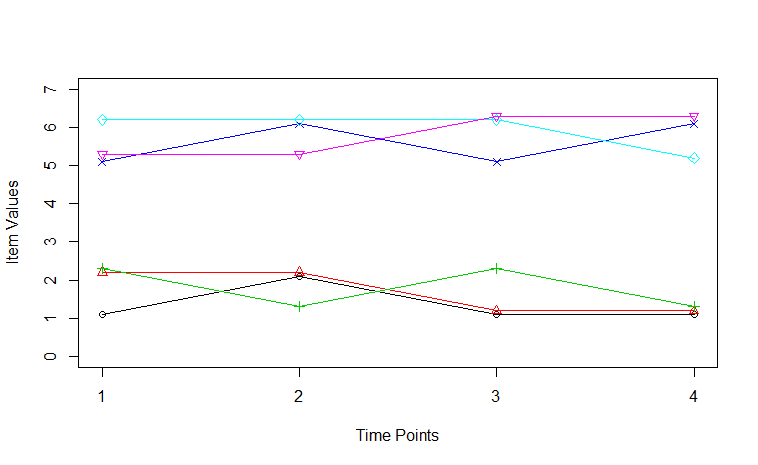
\includegraphics[width=0.75\textwidth]{images/chapter3/timeSeriesModel.png}}\\
		
		\subfigure[Focussing on the time points]{
			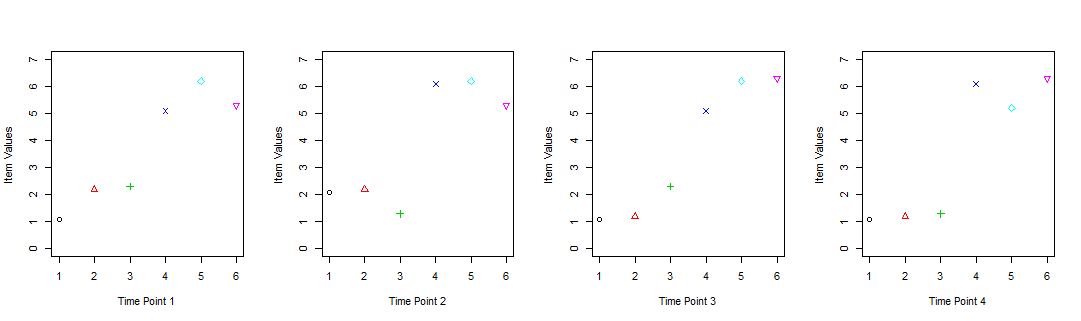
\includegraphics[width=.95\textwidth]{images/chapter3/timePointsModel.png}}
		\end{minipage}}
	\caption{Two different models focussing on temporal data. The first one focuses on the individual time series items while the second focuses on the time points and evaluates items according to their value in that time point. }
	\label{fig:temporaldatamodel}
\end{figure}

Before finding items' behavioural difference between any two time points, we had to find the categories for the behaviour of the items and how to group items according to these categories. It is important to categorise these behaviours so that neither nuance changes nor the shift of all groups are considered as a change in behaviour. For example, if we have two groups (poor and rich) of people's behaviour regards annual expenditure a slight change in the expenditure can not be considered as a significant change of behaviour, one that changes its status from poor to rich or vice versa. Moreover, a change of expenditure for the entire categories' might not be an indication of the change of behaviour. Instead, it may be due to inflation.

Another issue which could affect how to measure differences between time points in a data set with multiple time points (more than two time points) is what to consider as a normal reference behaviour of the item. By normal behaviour, we mean the general behaviour throughout in their data set. The first data point or any particular data points might not be a representative behaviour of an item. Therefore, this problem has also been addressed using different approaches in the study.


\section{Measuring Changes Over Time}
\label{MeasuringChangesOverTime}

As we mentioned in chapter two, the available methods for measuring changes over time focus on the overall changes in the clusters, agglomeration or the concentration of the of the data. These methods overlook the changes of the individual elements inside these clusters. In this section, we try to provide a method to quantify the magnitude of changes which reflect the change of items in a population. This is important to see the changes over time for individuals and the effect of an experiment. For example to measure the effectiveness of a new medicine or new teaching method can be quantified by measuring the change which individuals undergo in that process. In our case, it is required to measure the strategy change of players in public goods games which reflects the learning process that any player might undergo.

Measuring behaviour differences of items between time points requires three steps: The first step is to address time points, the second step is grouping similar behaviour and the last step is to find and measure the amount of differences between these time points. These steps will be addressed in the following paragraphs, and will be implemented and tested on the data in the next chapter.

The temporal data has to be split into separate time points. If the temporal data has discrete records of time, then each timestamp can represent a single time point. If the data set has continuous timestamps, then it might be converted to discrete using fixed intervals of time windows as used by many studies like \cite{Spiliopoulou2006}. It might be preferable that the time points have similar intervals between them so that the behavioural change measure M can represent the difference between any two time points in the same data set uniformly. Moreover, the items in each times point have to appear exactly once. This means if the items appear more than once in each time point an average value can be evaluated for the window. As an illustration consider $t \in T$ and the time intervals between [t-1, t] and [t, t+1] are equal which makes $m1 = \delta(t-1, t)$ and $m2 = \delta(t, t+1)$, so m1 and m2 can represent the two defined time intervals uniformly.

The second step is grouping similar behaviours of the items in the data so that we can identify each items' category of behaviour at every particular time points. As defined by Estivill-Castro \cite{Estivill-Castro2002} clustering is the task of finding groups of more homogenous (similar)members in a heterogeneous group of objects. Each time point is, thus, clustered using one of the clustering methods to find similarly behaving groups at each time point. The clustering algorithms used in the process of measuring the difference between time points in this study are K--means, PAM, and hierarchical clustering. Please refer to the previous chapter for the definitions and properties of these clustering methods.

Clustering items in each time point eliminate both the problems introduced in the previous section, namely potential minor changes in behaviour and the shift of all items in the same group. These problems are solved by clustering each time point separately without being influenced by other time points. Clustering will ensure that any values attributed by minor changes in items do not affect their membership in the group, and clustering each time point's data independently ensures that the entire movement of a group will not affect the measures of items' behaviour change. Please see Figure \ref{fig:lable1} for further illustration.

\begin{figure}[!h]
	\centering
	\subfigure[Original data set]{
		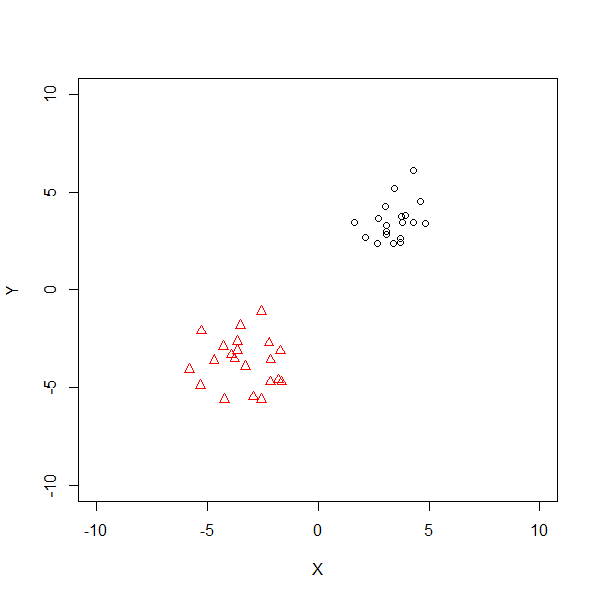
\includegraphics[width=0.32\textwidth]{images/chapter3/behaviourOriginal.png} \label{behaviourOriginal}
	} 
	\subfigure[Small behaviour changes]{
		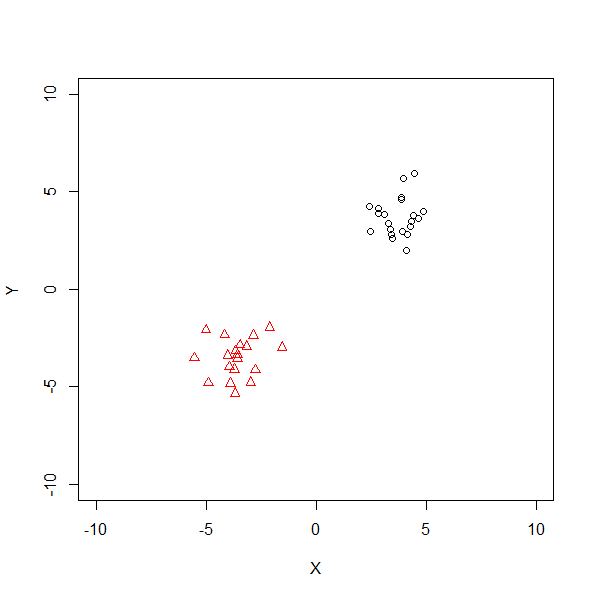
\includegraphics[width=0.32\textwidth]{images/chapter3/behaviourSmallChange.png}\label{behaviourSmallChange}
	}
	\subfigure[Entier group shift]{
		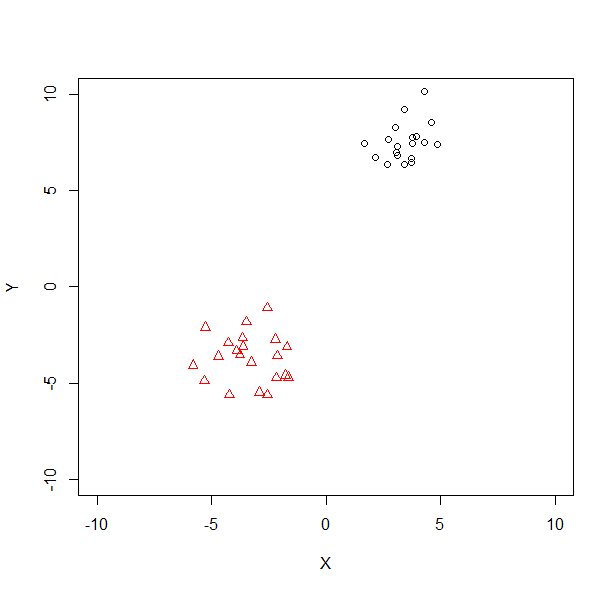
\includegraphics[width=0.32\textwidth]{images/chapter3/behaviourGroupMove.png}\label{behaviourGroupMove}
	}
	\caption{Three figures illustrating the small changes and the entire cluster move between two time points }
	\label{fig:lable1}
\end{figure}

The last step is to find the number of items which have changed their behaviour significantly so that they can be counted as they are in other groups or using the percentage of items' behaviour change. This means finding the $\delta$ function as described in the previous section. It is also possible to use AUC of ROC to find the difference between items' clusters in any two consequent time points by using cluster labels of t and t+1 instead of true class labels and predicted classes by a classification model as inputs to the AUC function so that it finds the difference between these two time points.

However, straightforward counting of items in clusters or using clustering labels as classes of the items might not be possible as it is hard to find one to one matching between clusters in consequent time points as described by Gunnemann et al. \cite{Gunnemann2011} and Xu et al. \cite{Xu2013}. Therefore, we use external cluster validity indices to compare between clusters of two time points and we replace the external labels with t cluster labels and guessed clusters by a clustering algorithm with t+1 cluster labels. This method can present a scalar measure as an indication of how much difference there exists between any two time points.

Multiple tests are implemented in Chapter four to check that this method can reflect the change in items' behaviour which is happening to the clusters (same behaviour grope). The tests include multiple external clustering indices as well as finding cluster pairs across time points so that other techniques like AUC can be tested. However to solve the problem of behaviour reference for the items as described in the previous section a new classification method is proposed. This will be elaborated on in the next section, and the detailed implementation of it in Chapter five.

 


\section{Temporal Rule-Based Classification}
\label{sec:Temporal-Rule-Based-Classification}
This section describes and explains the methodology for implementing the proposed rule-based temporal classification. As it has become obvious by now, this method targets temporal data with univariate or multivariate attributes. However, as stipulated by economists, the experts of public goods game, the rules should be presented in a simplified way, one human agents can understand. This provides simplicity and clarity with regards the rules for classification, and are expressed by using aggregated attributes which are derived from the temporal attributes. However, the final rules are formulated by considering of the temporal origin of these aggregated attributes.

\begin{figure}[!h]
	\centering
	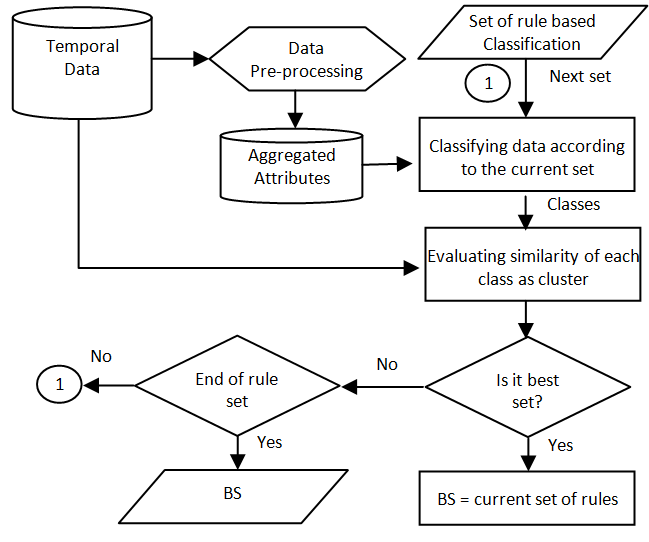
\includegraphics[width=0.7\textwidth]{images/chapter3/FlowchartTemporalClassification.png}
	\caption{The flowchart of the proposed rule-based temporal classification}
	\label{fig:FlowchartTemporalClassification}
\end{figure}

To achieve the conflicting goals of simplicity and consideration of the temporal attributes the classification process is divided into two main steps; rule generation and rule optimisation (as shown in the Figure \ref{fig:FlowchartTemporalClassification}). In the first step, rules are expressed using aggregated attributes of items with ranges of [min, max] values for each rule. In the second step, this range is optimised using temporal attributes to find the best cut in the provided range and select a single value for the rule.



This method might be both more effective and flexible than using aggregated attributes alone to classify items as it provides the flexibility to optimise rules in various ways: First, the aggregated attributes can be driven and optimised from different sets of items' temporal attributes. Second, it provides a way to include multiple inconsistent or overlapping ideas of experts on boundaries of classes, and by optimising these rules, the best possible classifier will be produced. This data set might be beneficial for cases when the items have both temporal and static data like expenditure behaviour (temporal) and career specialisation. Starting with a flexible model of rule-based classification and then determining the cut with an optimisation process might solve the problem of overfitting. This is because there is no requirement for the new data in the data set to follow the final cut of the old data, and the optimizer might generate slightly different values for final rules.


\subsection{Generating Initial Rules}
\label{sec:Generating-Initial-Rules}
Providing flexible rules for class boundaries is the first step of the temporal rule-based classification. To obtain these initial rules, this classification mainly relies on the experts of the field of knowledge for the data set and the intended items to be classified to obtain. As mentioned, the rules should be easy to read and interpret by human experts so that the provided rules are classifying temporal data sets on the basis of aggregated functions for each time series. However, the final result will also depend on the time dimension of the items.

There are numerous ways of using experts' knowledge to create classes boundaries to classify items. The most accessible method is to use their definition for the classes to create the rules for them. However, the definitions might not exist or can not be applied directly to the data. The second method involves asking their opinion on the rules of each class for the existing data. Experts' opinion can be developed interactively in multiple stages by creating profiles for items and viewing the results of previous rules that they have provided. Items' profiles illustrate their properties in a way that experts can create their opinion about the rules for the underlying data set.

To provide simple rules for classes so that they can be used by human agents to form definitions from them, complex temporal attributes have to be aggregated using one of the available functions such as the minimum value, maximum value, mean, mode, median and standard deviation. Each time series of the temporal data (items' specific data) can be aggregated using one or more of the aggregation functions so that sufficient quality and quantity of attributes are created to meet the requirements of the rules.

By flexible rules, we mean that each rule (or condition) has a range of candidate values which might fit it. The general form of the rule can be written as \textbf{$Attribute \left \{OP\right \} Value$}. The $Attribute$ can be any static property of the items either derived from a temporal attribute of the items using an aggregation function or other static values which are in the data set recorded separately from any temporal attribute. The $Value$ is a vector which contains all possible cuts between two classes. It can be expressed as [min, max] pairs to represent the beginning and the end of the range of the cut between two classes in its dimension. The $ \left \{OP\right \} $ can be any of the comparison operators like $\left \{\leqslant , \geqslant , < , > , = and \neq \right \}$. The classes might have multiple conditions which represent the boundaries of the class. These conditions can be combined using logical $and//or$ operators. Figure \ref{fig:illustrationofRules1} shows an illustration for ranges of values created by using flexible rules for two attributes to split items into different classes.

\begin{figure}[!h]
	\centering
	\includegraphics[scale=0.55]{images/chapter3/illustrationofRules1.png}
	\caption{An illustration of the ranges which splits between neighboring classes. These ranges will be changed into crisp lines after optimisation process}
	\label{fig:illustrationofRules1}
\end{figure}

The range value [min, max] of two neighbouring classes for the same attribute might overlap due to the differences in experts' opinions about each class limits or from slightly different definitions for each class. To prevent an item possibly falling into two classes at the same time due to the overlapping problem, the classes have to be prioritised. This means when an item fulfils the condition of the higher priority class, there is no need to check for lower priority classes. This might be done using a nested if-else statements. Moreover, the lowest priority class might be without any condition because if an item does not fall into any class category, they might be in the last one. However, if conditions are not used for the least priority class, a careful design for higher priority classes should be undertaken to prevent ambiguity or it might be better to consider a non-exclusive label for the last class like others or not-determined.


The next step focuses on changing the ranges of values of rules into single values by using temporal attributes of the items.



\subsection{Optimising Initial Rules}
\label{sec:Optimising-Initial-Rules}

The result of the first step of temporal rule-based classification is creating generalized rules with indeterminate boundaries of classes for classifying items. In the second stage, the boundaries of classes will be converted from vector ranges of values to scalers with a single value. Figures \ref{fig:illustrationofRules1} and \ref{fig:illustrationofRules2} should be compared to provide an illustration of the task for this step of classification. To link temporal features of the items and their corresponding non-temporal aggregate attributes, which are generated to create rules for classification, this stage will use temporal data to decide on choosing a scalar among the provided range of values. 


\begin{figure}[!h]
	\centering
	\includegraphics[scale=0.5]{images/chapter3/illustrationofRules2.png}
	\caption{An illustration for the boundaries of classes and how the ranges are converted into line separators.}
	\label{fig:illustrationofRules2}
\end{figure}


For each provided vector in the rules, this step finds the best scalar to divide adjacent classes. The point is considered as the best dividing point when it produces the most compacted classes of items at every time point using the temporal features to measure the distance between items. This process can be accomplished by iterating through all possibilities of the value ranges for the rule-based classifiers, as implemented in chapter five or using a heuristic search algorithm as implemented in chapter six using Differential Evolution. See algorithm \ref{alg:bruteForceOptimization} for the brute force method to determine the best classifier.

\begin{algorithm}[!h]
	\SetAlgoLined
	\KwData{Temporal data and aggregated attributes to represent classification rules}
	\KwData{R= set of classification rules which includes discrete value rages}
	\KwData{minCost = Inf}
	
	\ForEach{r in R}{%
		c = classify(PG, r)\;
		cost = calculateCost(c)\;
		\If{cost < minCost}{
			minCost = cost\;
			bestClassifier = r\;
		}
	}
	print bestClassifier\;
	
	\Fn{calculateCost (C)}{
		\ForEach{t in Periods}{%
			\ForEach{c in Classes}{%
				costs.append(CM(ct ) * count(c))\;
			}
		}
	}
	
	\caption{Using brute force to optimize rule ranges}
	\label{alg:bruteForceOptimization}
\end{algorithm}


The classification step uses provided rules with a single value for each range of the values. If the value ranges are continuous, they should be discretised into acceptable discrete values. Selecting the acceptable discretisation intervals is a specific area and underlying data which can be decided by consulting area specific experts. By iterating though all values, the classifier tries values to classify underlying data labels items accordingly and sends them to the next step to be evaluated.

The evaluation step uses item labels provided by the classifier of the previous step and uses temporal attributes to evaluate compactness of the classes in each time point. The compactness of classes can be calculated using different criteria, such as standard deviation, internal clustering indices or measures of distance. To calculate a measure for compactness, we created a weight function to be used as a cost function for evaluating the goodness of every classifier, and then returned the best classifier as a final result for the optimisation process. After this process, the items can be classified by the best rule-based classifier values.

For a generalised optimisation process, it can be assumed that experts' definitions and consultations produce N classes for items have to be classified using aggregated attributes of temporal data, producing D of possible classifiers of rule-based classification for different ranges of values for each class. Our task is to select the best classifier among a set S of size D classifiers, hence reducing each provided separator range between neighbouring classes into a single line of separation, using the temporal attributes of T time points. A cost function  for each $C \in S $ can be produced using any \acrfull{cm} that measures the goodness of classes in each time point. The can be defined as: 
\begin{equation*}
	f(C) = \sum_{t=1}^{T} \sum_{n=1}^{N} CM(c_{n}^{t}) \times \left | c_{n} \right |
\end{equation*}
where $ \left | c_{n} \right |$ is number of items in each class to prevent creating single big classes. The classifier with the smallest $f(C)$ value can be considered as the best classifier among S.

\subsubsection{Evolutionary Algorithms}

In nature, evolution consists of two steps, selection and random variation. A population of individuals living in an environment do not have the exact same traits. Some of these traits might be more advantageous and fit better for that specific environment. These individuals have more chance of surviving and producing offspring while others will die out. This fitness for the experiment is the natural selection. The surviving individuals will carry their traits through to the next offspring of the population though DNAs. However, the offspring of the surveyed individuals might not have the exact DNAs as their parents because the operation of replicating DNAs consists of randomly crossing both parents' DNAs. The operation itself might result in some errors which might lead to new mutations. This operation of creating new traits through random crossovers and mutations is called random variation which might be more beneficial (best fitting) for the environment
 \cite{Back1997}. 

Evolutionary Algorithms are inspired by the natural evolution in biology. Given that, they comprise the same steps as their natural counterfeits. There are many flavours of the algorithm with slightly different implementations. However, all of them have the same basic components as shown in shown in Figure \ref{fig:EALifeCycle}, this figure represents the general flowchart for evolutionary algorithms \cite{Eiben2015}.

\begin{figure}[!h]
	\centering
	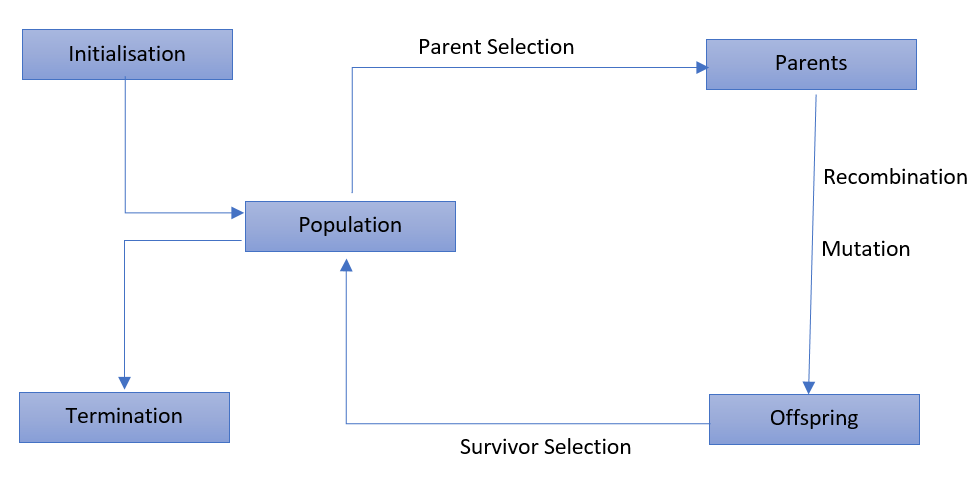
\includegraphics[scale=0.4]{resource/EALifeCycle}
	\caption{General operations of evolutionary algorithms. 
		From Eiben et al. \cite{Eiben2015}.}
	\label{fig:EALifeCycle}
\end{figure}

In their book \cite{Eiben2015} Eiben and Smith listed the components of evolutionary algorithms as follows: 
\begin{itemize}
	
	\item \textbf{Representation}: Is the operation of mapping the real world into the Evolutionary Algorithm world. This process consists of translating phenotypes into genotypes which are typically accomplished by the domain experts.
	
	\item \textbf{Fitness Function}: Also known as evaluation function, this function assigns a quality measure for each genotype helping the process of selecting the desired behaviours from the population. Hence this function acts as the environment for a population which favours certain phenotypes according to their genotype. The most fitted behaviours or phenotypes represent the solution for the underlying optimisation problem of the evolutionary algorithm.
	
	\item \textbf{Population}: The population consists of individuals carrying different genotypes. These genotypes represent a possible solution for the issue of optimisation. In most evolutionary algorithms, the population size remains constant, which means that after producing a number of the new generation, the same amount of the individuals will be eliminated for the next phase of the population.
	
	\item \textbf{Parent Selection}: Is a mechanism of selecting individuals to undergo the operation of generating a new individual (child). This process is statistical; this means, the individuals of a higher quality will be selected at a higher rate than low-quality individuals. Nevertheless, the low-quality individuals also have a high chance of being selected, so that the search does not become greedy and stuck in a local optimum.
	\item \textbf{Variation}: Variation consists of two different operations; recombination and mutation:
	\begin{itemize}
		\item \textbf{Mutation}: Is a stochastic process which changes some values of the selected children's' genotype to mimic the natural mutation. This process might produce individuals with better characteristics than the available population and helps to avoid local optima \cite{Grefenstette1986}.
		\item \textbf{Recombination}: Also called crossover, it is a process of creating the genotypes of new offspring using random parts of the selected parents' genotypes.
	\end{itemize}
	\item \textbf{Survivor}: Also called replacement, this is the process of selecting some new offsprings to survive and pass their genotypes to the next generation. This process, with parent selection is responsible for keeping the population size constant.
\end{itemize}



\subsubsection{Differential Evolution}

Differential Evolution is introduced by Storn et al. \cite{Storn1997} as a type of evolutionary algorithms. As described by Storn et al. \cite{Storn1997}, this method can optimise nonlinear, none-differentiable continuous and multidimensional space function.

The obvious difference between differential evolution and other evolutionary algorithms like genetic algorithms is it can operate on real numbers rather than integers. Furthermore, differential evolution employs the components of evolutionary algorithms in a different way as described below \cite{Storn1997}:

\begin{itemize}
	\item \textbf{Initialisation}: The initial population must cover the entire search space. This can be accomplished by randomly assigning values for the individuals. The random values have to be in the range of the minimum and maximum values of the search space.
	
	\item \textbf{Mutation}: Mutation is accomplished by creating a mutant vector from individuals of the population. This is called target vector. The mutant vector is a result of a target vector and the difference of two vectors which might be chosen randomly or from the best quality individuals.
	
	\item \textbf{Crossover}: Is the operation of copying a fraction of the mutant vector to its corresponding target vector. This ratio of the copy is constant and can be controlled by the end user. If the values of the resulting individual exceed the range of the search space, this individual will be reinitialized. 
	
	\item \textbf{Selection}: In this stage, the fitness value of the target vector and resulted vector will be compared. The best fitted vector will survive and the other one will be eliminated.
\end{itemize}


In chapter six of this study, we will use Differential Evolution with the proposed classification method to optimise a classifier from a pool of classifiers provided by domain experts. The reason behind choosing differential evolution for optimising the proposed classification method is its characteristics as described by Stor et al. \cite{Storn1997}. It has been successfully implemented with multiple data mining methods as listed by Das et al. \cite{Das2011}. Furthermore, Tusar et al. \cite{Tusar2007} proved that for most cases differential evolution is more efficient and effective than other genetic algorithms that use multiple benchmarks.


\section{Statistical Measures and Tests}

In this thesis, multiple statistical measures and tests are used for different reasons such as measuring the spread of a variable or finding similarities between resulting samples. In the following subsection, we briefly introduce some of these statistical tools. They are used across multiple chapters of the thesis. Other statistical measures, when used, will be introduced in their respective chapters.


\subsection{Variance and Standard Deviation}

Variance measures the spread of random variables around their mean. It uses the sum of squared difference between readings and the mean to calculate the amount of spread \cite{Kenney1947}. For the random variable $X$ which consists of $N$ readings and its average is $\overline{X}$ its variance ($\sigma^{2}$) will be:

\begin{equation*}
	\sigma^{2} = \frac{\sum (X - \overline{X})^{2}}{N -1}
\end{equation*}

\acrfull{stdiv} measures spread of variables as it is calculated as a square root of variance $\sigma^{2}$. It is denoted as $\sigma$. In this thesis, we refer to standard deviation as StDev. To calculate the standard deviation \cite{Kenney1947}:
\begin{equation*}
	\sigma = \sqrt{\sigma^{2}} = \sqrt{\frac{\sum (X - \overline{X})^{2}}{N -1}}
\end{equation*}


\subsection{Interquartile Range}

\acrfull{iqr}, also known as H-spread, is the range of the middle half of a random variable. For a ranked variable, the total range of the data is divided into four quarters that is Q1, Q2, Q3 and Q4. Each quartile consists of 25\% of the readings. The Interquartile Range can be calculated as $IQR = Q3 - Q3$ \cite{Ross2010}. This range can be considered as another measure of spread. However this IQR ignores the outliers and extreme readings of the variable.

Quartiles can be graphically represented as boxplots. Normally a boxplot has a vertical line representing the range of values of the readings in the variable with horizontal lines cutting through the main vertical line showing the range of each quartile. The second and third quartile are placed in a box demonstrating the IQR of the variable as shown in Figure \ref{fig:boxplotIllus}.

\begin{figure}[!h]
	\centering
	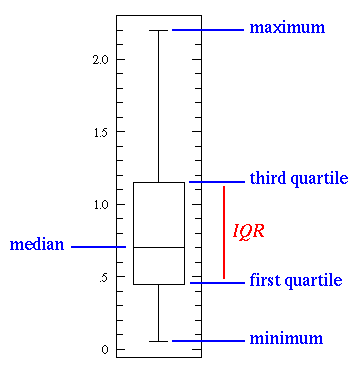
\includegraphics[scale=0.5]{images/chapter3/boxplots.png}
	\caption{An illustration of different parts of a boxplot showing quartiles and their interquartile range. From Kirkman \cite{Kirkman1996}}
	\label{fig:boxplotIllus}
\end{figure}

\subsection{Wilcoxon Test}

The Wilcoxon ranked test is a statistical method to test the null hypothesis of median equality between two paired variables \cite{MCDONALD2008}That is, the same sample has been used for two different experiments, in contrast to the t-test, this test does not assume normality of distribution for data which, thus, makes it a non-parametric test. However, it assumes that data is symmetric around median \cite{MCDONALD2008}. 

\subsection{Friedman Test}

The Friedman Test is a statistical non-parametric ranked test which can treat multiple dependent samples sets \cite{Ross2010}. The null hypothesis of the Friedman Test is that there is no difference between variables. The null hypothesis can not be rejected if the result of the treated testes is higher than the pre-appointed significance value \cite{Friedman1940}. Non-parametric means that this test does not assume normality in the sample (that is, the condition of using this test is the data require a normal distribution around the mean) \cite{Ross2010}.

This study uses the Friedman test to find the significance of the differences between the results of the proposed methods, and other available methods of classification and measuring changes over time. Given the characteristics of the Friedman test, multiple samples can be compared without assuming normality. Moreover, this test is used in data mining and data analysis to compare the results of different algorithms of classification \cite{Demsar2006} and methods of concept drift \cite{Goncalves2014}.


\section{Used Data Sets in This Study}
\label{section:Used-Data}

In this study, four data sets are used for different purposes. A synthetic data is used to evaluate the fitness of the external clustering validity to measure the differences in the data. Two data sets of the public goods game are used to measure the players' behaviour change over time and classify them using the proposed method. The final data set is that of a stock market, which is used to test whether the proposed methods can be generalised to other cases or not.



\subsection{Creating a Synthetic Data}
\label{CreatingaSyntheticData}

To check the validity of our method for quantifying behaviour changes of items over time, we create a simple 2D data set. These items are agglomerated to form four distinct clusters with their centres separated around the origin (0, 0) point. The original data set is mutated to create the next time point and to simulate the behaviour change of items.

We used the mlbench.2dnormals method of package mlbench of R language which is developed by F. Leisch and E. Dimitriadou \cite{mlbench210} to create the original data set\footnote{The R code for creating this synthetic data set is available at https://goo.gl/8DBuII}. The data set contains 500 (x, y) items (points) separated randomly among four clusters. Each cluster's centre is placed on a circle with a radius equal to 6, and its centre is point of origin (0, 0). Items inside each cluster have a Gaussian distribution and spread from its centre with 1.5 of standard deviation. Please refer to Figure \ref{fig:synthesisData_first} to see the produced data set and its items distribution among clusters.

To create the effect of time passing and items behaviour change, the set is mutated to create the next time point. By repeating the mutation process on the previously mutated data set, multiple time points are created (for our tests, 20 time points are created). For the data set DS for time t, D(t+1) = D(t)' where D(t)' is the mutated version of D(t). 

Two methods are used to mutate the data and generate the next time point. First, by changing the x and/or y coordinates sign value from positive to negative or vice versa of a randomly selected number of items. This change of sign make items jump from one cluster into another. The first change of data can be considered as a big change, which leads items to change their behaviour significantly. The second kind of change is introduced to all items in the data set by slightly changing their x and y values so that they will jiggle from their position without leaving the cluster. The amount of jiggle depends on the x and y values of the item as each item will be displaced with a random value range from 1\% to 2\% of its original value. Please refer to Figure \ref{fig:synthesisData_mid} and \ref{fig:synthesisData_last} for the mutated data sets which represent the middle and last time points for the temporal data set.

\begin{figure}[t]
\centering

\subfigure[First time point]{
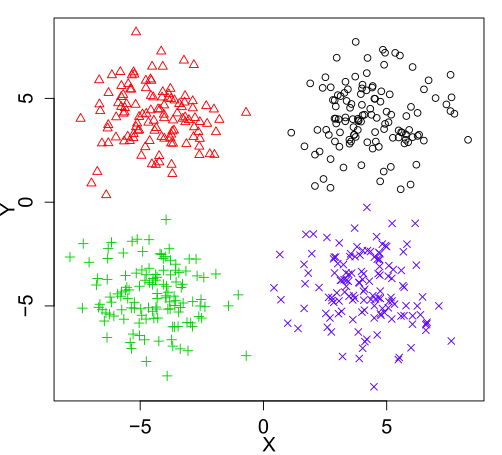
\includegraphics[width=0.31\textwidth]{images/chapter3/synthesisDataFirst.png}\label{fig:synthesisData_first}}
\subfigure[Middle time point]{
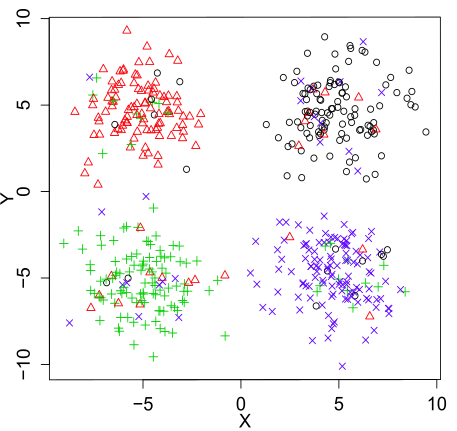
\includegraphics[width=0.30\textwidth]{images/chapter3/synthesisDataMid.png}\label{fig:synthesisData_mid}}
\subfigure[Last time point]{
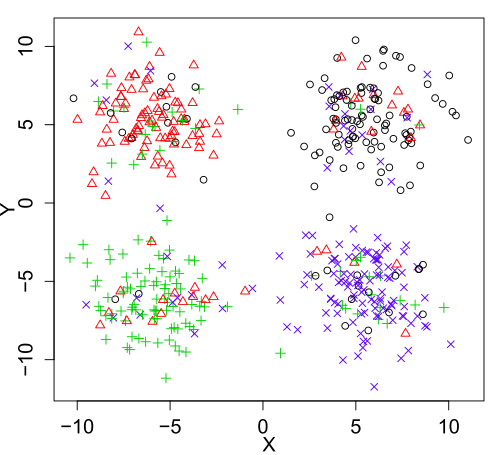
\includegraphics[width=0.30\textwidth]{images/chapter3/synthesisDataLast.png}\label{fig:synthesisData_last}}
\caption{Three time points (first, middle and last) from the overall created 20 time points. The first time point which contains 500 items separated into four clusters is the original data set other time points are created by mutating (jumping) items of four clusters from one cluster into another.}
\label{fig:synthesisData}
\end{figure}

\subsection{Public Goods Games Data}
\label{PublicGoodsGamesData}
There are many variations and set-ups for the public goods game experiment (cite), However, the data which has been used in this study is collected through experiments conducted by Fischbacher et al. \cite{Fischbacher2012}. Their experiment for public goods game consists of two sub-experiments; \gls{P-Experiment} and \gls{C-Experiment}, both of which every participant (player) has to accomplish. In the following sections, we will explain how these two sub-experiments are conducted, and then describe the collected data which will be used in later chapters.

\subsubsection{Game Set-up}

Prior to each sub-experiment of P-experiment and C-Experiment, experimenters explain the rules of the game for the participants so that they understand the rules, and how their decision will affect their result and the number of points available. Participants should answer a number of control questions correctly to demonstrate their comprehension of the game. Experimenters make every effort to ensure that the players are paying attention and playing thoughtfully by rewarding them extra points for correct guesses and well-thought out decisions during the game.

In P-experiment, four players start the game with 20 points each in their private account and they can contribute any amount they deem necessary to a project which represents public good. The amount which they do not contribute in the project will be kept only for the players themselves. The collected amount from the project will be distributed among all players regardless of their contribution to the project. The amount of points each player can accrue from the project is determined by this equation:

\begin{equation*}
Player Share From Project = Total Amount Of All Players Contribution * 0.4
\end{equation*}
So that each players total point after the game will be:
\begin{equation*}
Player's Points = (20 - Contribution In The Project) + Player Share From Project
\end{equation*}

In P-Experiment, players are asked to make two kind of contribution; conditional and unconditional. In conditional contribution, players are asked to decide what amount of points they wish to contribute in response to the rounded average of other players' contributions. This contribution will be filled out by the player in a form called the contribution table as shown in Figure \ref{fig:pgg1RoundOfGame}. The unconditional contribution players will input the amount of contributions which they require in a single field without any conditions. Please see Figure \ref{fig:pgg20Questions} for unconditional contribution.

\begin{figure}[!h]
	\centering
	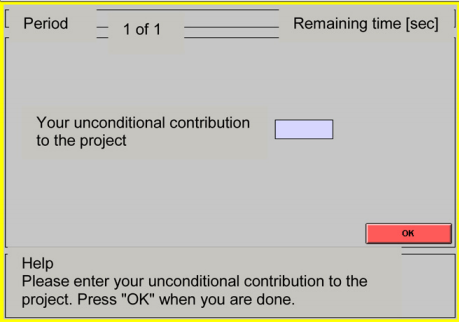
\includegraphics[scale=0.55]{images/chapter3/pgg1RoundOfGame.png}
	\caption{P-experiment's unconditional contributions user interface. which the user can enter their amount of contribution.
		From Fischbacher et al. \cite{Fischbacher2012}}
	\label{fig:pgg1RoundOfGame}
\end{figure}
\begin{figure}[!h]
	\centering
	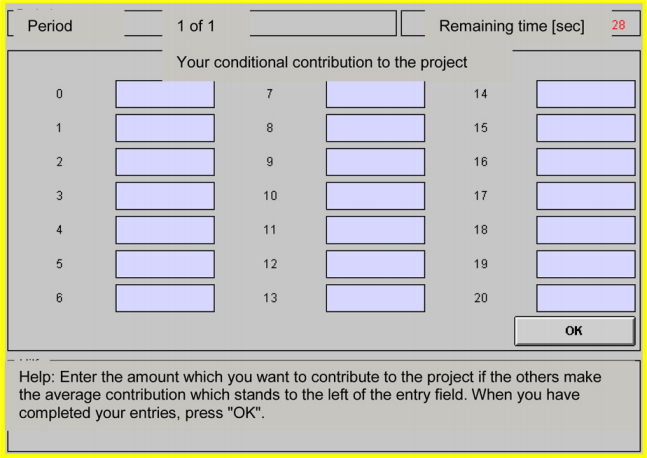
\includegraphics[scale=0.45]{images/chapter3/pgg20Questions.png}
	\caption{P-experiment Contribution table user interface in which the user can enter their contribution for all possible conditions. 
		From Fischbacher et al. \cite{Fischbacher2012}}
	\label{fig:pgg20Questions}
\end{figure}

For each player, only one of the two contributions will be selected by the computer as their final contribution to the project. One of the four players' conditional contribution will be randomly chosen to be used as their final contribution. while for the other three players their unconditional contribution will be used. This random selection of players' contributions is one of the mechanisms that experimenters have used to make sure that players are thinking thoroughly about their decision for the contribution to the project.

When the P-experiment is completed, players start C-experiment. C-experiment is similar to a repeated sequence of unconditional contribution except

this time the player, in addition to their own contribution, will be asked to guess other players' rounded average of contribution. After each round of the game, players will be notified of their total points in that particular game. The sequence length of the games can vary from one experiment to another. In this study, we will use data sets with 10 and 27 series of rounds of the game. In each round, four different random players will play the game so that players can not predict others' contributions in advance. Players will gain extra points if they make correct guesses about other players' rounded contributions. They will, therefore, not fill in the boxes
 randomly. Please refer to Figure \ref{fig:pgg10RoundOfGame} for the interface of C-experiment.

\begin{figure}[!h]
	\centering
	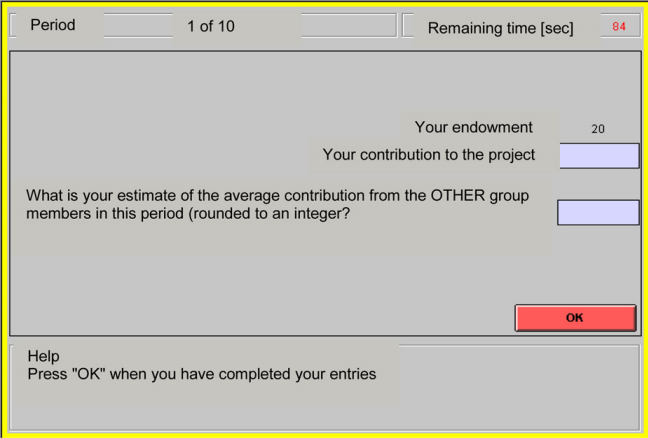
\includegraphics[scale=0.45]{images/chapter3/pgg10RoundOfGame.png}
	\caption{C-experiment user interface has two fields. One for the amount of players own contribution and the other for guessing other players rounded average contribution. From Fischbacher et al. \cite{Fischbacher2012}}
	\label{fig:pgg10RoundOfGame}
\end{figure}

\subsubsection{Data Set Attributes}

To measure and classify the behaviour of players in public goods games, this study used two different data sets. These experiments are conducted on different samples of players, so the first data set has 140 players and the second data set 128 players. These data sets have the same attributes and follow exactly the same experiment procedures, except for the P-experiment length, as the first one consists of 10 rounds while the other has 27 rounds.

Due to the limitations in space and equipment, all players in these experiments did not play at the same time. Instead they were distributed into multiple sessions. However, each session consisted of sufficient number of players meaning that the random selection of each four players playing with each other is unbiased. The behaviour of each player will not be affected by the session which they are in, as they are experiencing the game for for the first time and develop their understanding of the different strategies during P-experiment. Therefore, we are able to consider that the experiment has been conducted in one big session with all players playing the rounds of the P-experiment at the same time. This means for the first data set, we consider that all 140 players have played the first round of P-experiment at the same time.

The attributes of the data sets can be divided into two types the temporal and non-temporal attributes. The temporal attributes are generated in the P-experiment as it contains multiple rounds and non-temporal attributes are generated in C-experiment. The following is the list of all the attributes of the data sets. Please notice that the temporal attributes are underlined:
\begin{itemize}
\item \textbf{Idtyp}: labels for players categories assigned by experts. The categories are: conditional contributors = 1, free riders = 2, triangle contributors = 3, and others = 4. These categories are generated depending entirely on the b0-b20 attributes. Figure \ref{fig:percentage} shows the average contribution behaviour of players in each category. Please refer to the previous chapter for the detailed description of these categories.

\item \textbf{Idsubj}: a unique identifier for each player during both C and P experiments.

\item \textbf{b0-b20}: twenty one attributes representing the contribution table for each player as their response in C-experiment to every possible rounded average of other players' contribution.

\item \textbf{u}: the unconditional contribution of the player for C-experiment during the actual game.

\item \textbf{\underline{Predictedcontribution}}: Players' prediction about other co-players rounded average of contribution to the project.

\item \textbf{Period}: the session number for P-experiment. As P-experiment for each player consists of multiple rounds, each players' playing times are recorded to keep track of the number of games played.

\item \textbf{\underline{Contribution}}: players' actual contribution to the project in each round of the P-experiment.

\item \textbf{\underline{Belief}}: players' beliefs about other players average contribution in each session.

\item \textbf{\underline{Otherscontrib}}: Other co-players' rounded average contribution.


\end{itemize}

\begin{figure}[!h]
	\centering
	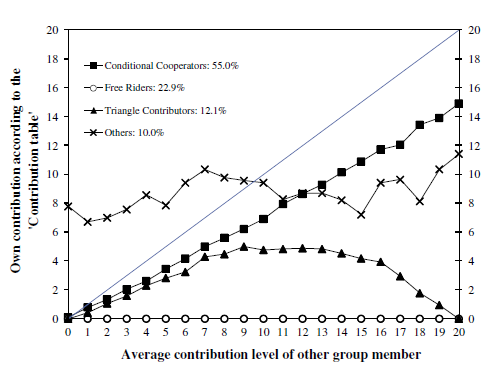
\includegraphics[scale=0.45]{images/chapter3/percentage.png}
	\caption{Four type of players average own contribution according to co-players average contribution }
	\label{fig:percentage}
\end{figure}

\subsubsection{Preliminary Behaviour Analysis of the Players}

As mentioned before, experts use C-experiment data to classify players' strategies. However, we are using the P-experiment data to classify players' behaviour over time and measure their overall change in contribution. So before starting the analysis for classification, it is beneficial to see the general trend of players' behaviour over time and gain an overall idea about them. Heat maps are used to identify the density of players' contribution at each round of the game with regards their beliefs about other co-players' contribution. The heat map shows the percentage of players who have the same contribution and belief. The more similar the behaviour is of the players, the darker the box of that value becomes. 


Figures \ref{fig:contribution1}, \ref{fig:contribution2} and \ref{fig:contribution3} represent players contribution-belief heat maps generated for the first, mid and last rounds of the first data set. As can be noticed, the overall players' contribution for the project and their belief of co-players contribution drop significantly from the first to the last round. However, it can also be noticed that the players contribution drops faster than their belief as more dark boxes can be seen at the bottom of Figure \ref{fig:contribution2}. This indicates players are starting to contribute less than what they believe the other players will contribute to the project to obtain more points from the project than contributing in it.

\begin{figure}[!h]
	\centering
	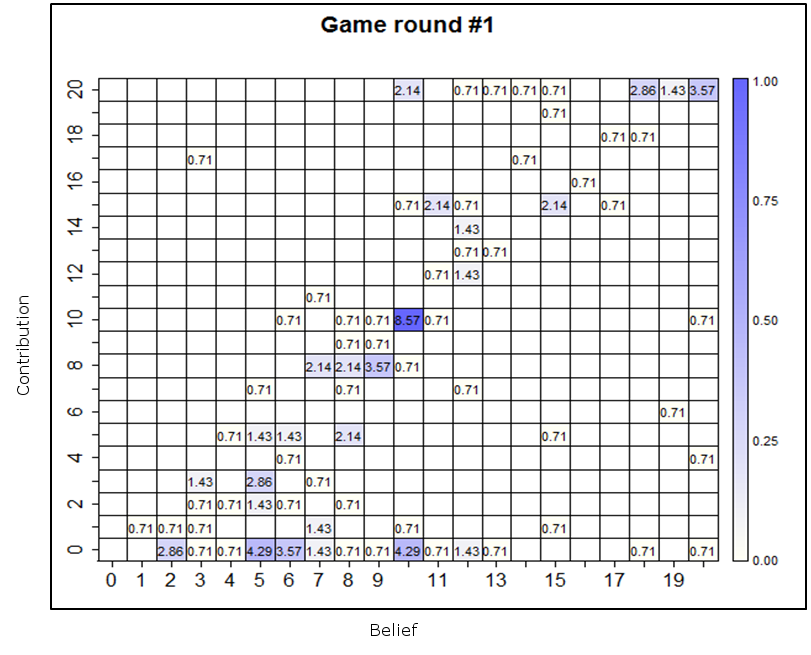
\includegraphics[scale=0.35]{images/chapter3/HeatMapContribution1.png}
	\caption{Heat map for players contribution according to their belief in round 1}
	\label{fig:contribution1}
\end{figure}
\begin{figure}[!h]
	\centering
	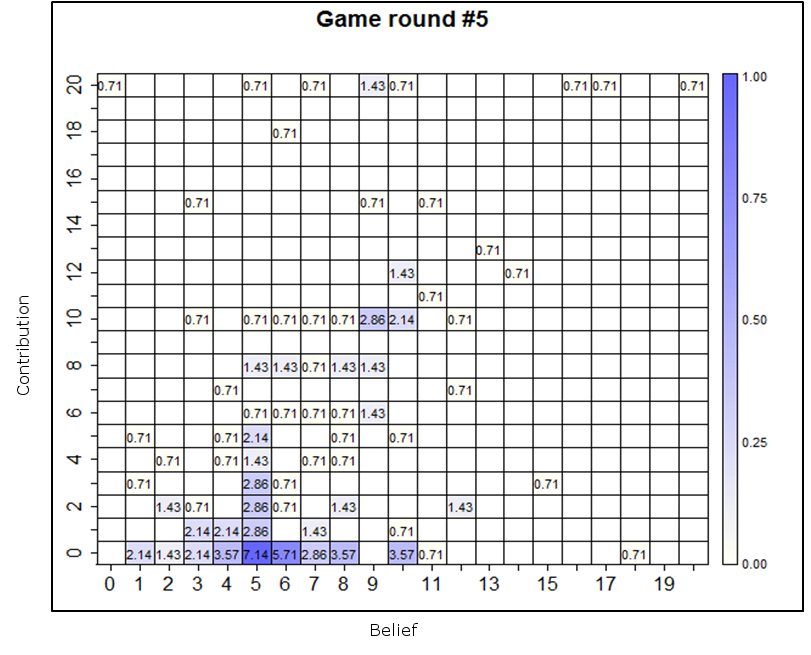
\includegraphics[scale=0.35]{images/chapter3/HeatMapContribution5.png}
	\caption{Heat map for players contribution according to their belief in round 5}
	\label{fig:contribution2}
\end{figure}
\begin{figure}[!h]
	\centering
	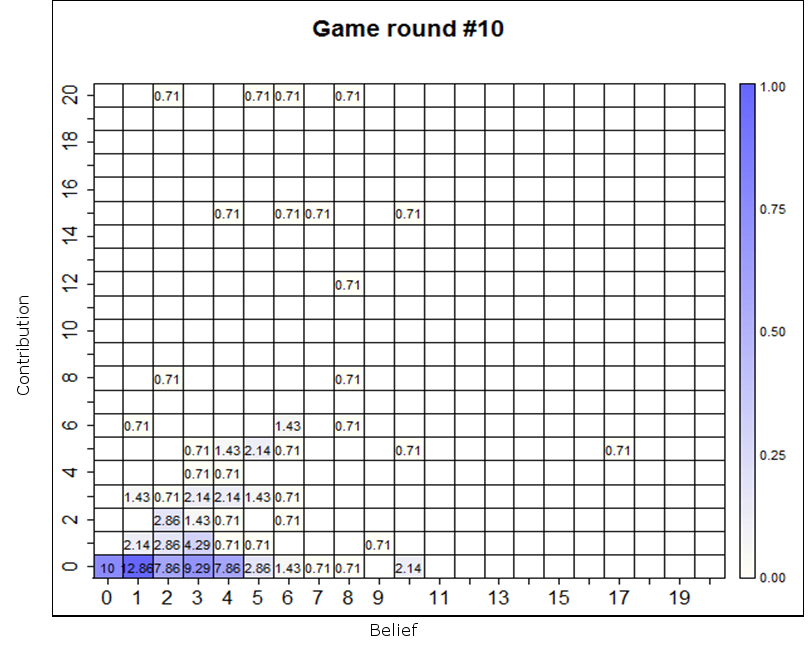
\includegraphics[scale=0.35]{images/chapter3/HeatMapContribution10.png}
	\caption{Heat map for players contribution according to their belief in round 10}
	\label{fig:contribution3}
\end{figure}

\begin{figure}[!h]
	\hfill{\begin{minipage}{\dimexpr \textwidth-2\fboxsep-2\fboxrule}% maximum allowed
			\centering
			\subfigure{
				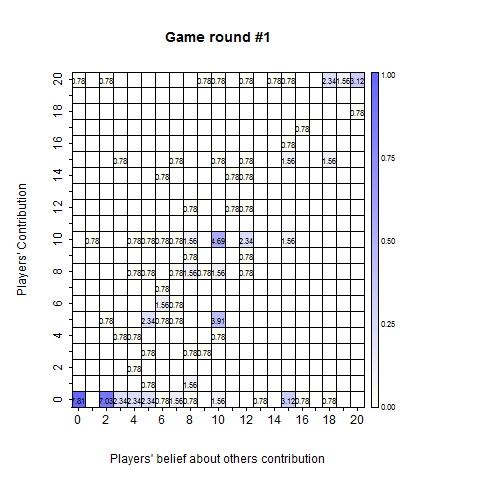
\includegraphics[width=0.45\textwidth]{images/chapter4/heatMap27/heatMap27_1.png}
			}
			\subfigure{
				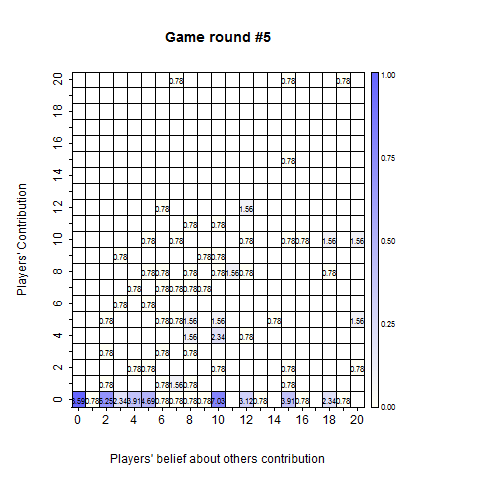
\includegraphics[width=0.45\textwidth]{images/chapter4/heatMap27/heatMap27_5.png}
			}\\
			\subfigure{
				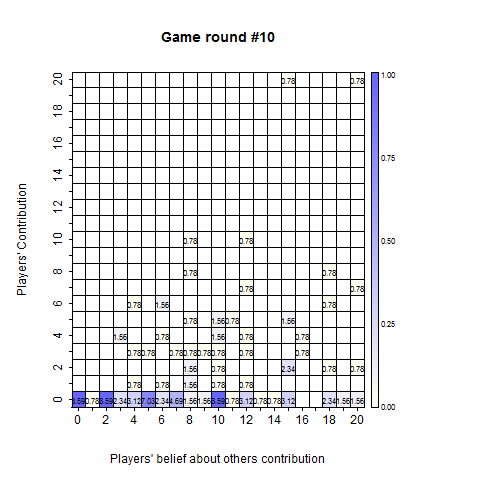
\includegraphics[width=0.45\textwidth]{images/chapter4/heatMap27/heatMap27_10.png}
			}
			\subfigure{
				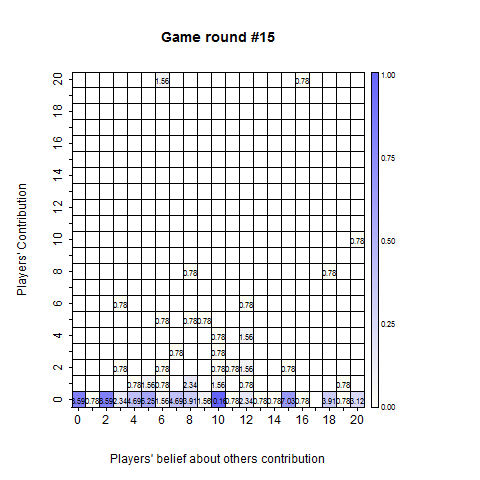
\includegraphics[width=0.45\textwidth]{images/chapter4/heatMap27/heatMap27_15.png}
			}\\
			\subfigure{
				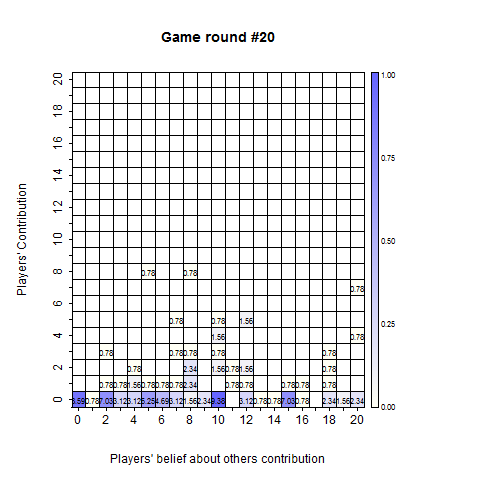
\includegraphics[width=0.45\textwidth]{images/chapter4/heatMap27/heatMap27_20.png}
			}
			\subfigure{
				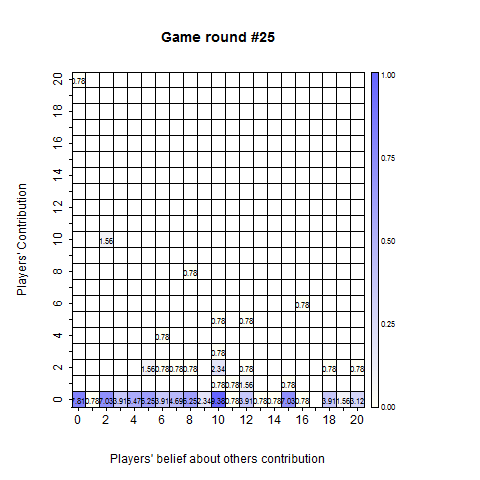
\includegraphics[width=0.45\textwidth]{images/chapter4/heatMap27/heatMap27_25.png}
			}\\
			
		\end{minipage}}
		\caption{Selected heat maps for players contribution according to their belief in rounds 1, 5, 10, 15, 20 and 25 in the 27 rounds data set}
		\label{fig:contributionRound27}
	\end{figure}

\subsection{Stock Market Data}
 We further tested the proposed classification and measuring methods using different data sets with similar required properties. The stock market data set was chosen as it contains elements (stock) in a temporal data with varying behaviour (prices). One advantage of the stock market data set is that we can select a larger set of unique items to be classified and longer time points to observe their behaviour change. This might be a good way to test the proposed methods to their full extent. However, the downside of the collected stock market data is that there are no pre-classified labels for the items in the data to be able to compare with in our findings. Therefore, we should rely on some other measures to evaluate our results.

\subsubsection{Data Harvesting}

For this study, we have selected \acrfull{sp500} stock market to run our tests as they contain a sufficient amount of items at each time point (502 items \cite{Goings2014}). In addition, it is publicly listed and this enables us to harvest long periods of their data freely. S\&P\,500, or historically known as Composite Index \cite{TheEditorsofEncyclopædiaBritannica} is designed to represent the large cap for domestic companies in United States \cite{Britannica2015}. This index comprises very diverse stocks which can be considered as a better representation of the U.S. market than Dow Jones . The large cap, in this context, refers to companies with more than 10 billion dollars worth of stocks \cite{Editors2016}.

We used the available symbols for the companies listed in S\&P\,500 index from \href{http://www.cboe.com/products/snp500.aspx}{cobe} website as it is specialised in market analysis. Symbol (or ticker) is a standard representation for a company in the stock market. We have used the list of S\&P\,500 symbols to download historic data of the companies from \href{https://uk.finance.yahoo.com/}{Yahoo Finance} website using an R script \footnote{The Symbols list, R script for fetching the data and manipulating it, and a sample of the data are available at \href{https://goo.gl/U0STqJ}{https://goo.gl/U0STqJ}}.

A sample data for all companies listed in S\&P\,500's index from 1-1-2015 to 1-7-2015, which represents a half year, are collected from the Yahoo finance website. The number of time points which are collected for this time period is 125 days, and the attributes for the collected data are:

\begin{itemize}
	\item \textbf{Date}: The date of the stock price. Each date can be considered as a time point and converted to a sequence of integer numbers.
	\item \textbf{Symbol}: The standard symbol which identifies companies' stocks.
	\item \textbf{Open}: The price of the stock at the opening time for that date.
	\item \textbf{High}: The highest price that the stock reached on that date.
	\item \textbf{Low}: The lowest price that the stock hit at that date.
	\item \textbf{Close}: The price of the stock at the close time of stock market at that date.
	\item \textbf{Volume}: The number of shares which are traded at that date.
	\item \textbf{Adj.Close}: The closing price of each stock might be amended to that date because of one of multiple reasons that might affect the price such as Stock Splits, dividends and Rights Offerings \cite{EditorsInvestopedia2016}. 
\end{itemize}

\subsubsection{Data Preprocessing}

The harvested data should be cleaned and pre-processed before using it to test the proposed methods. The unknown fields should be handled properly so that they do not subsequently affect the algorithms. The unknown fields are not the only problem as the stock price values from one company to another varies significantly. As this may affect the classification process, they should be normalised. Moreover, for the sake of simplifying the classification rules later, it is advisable to convert normalized data into integers. Table \ref{tab:stockdata} shows a sample of the data with its headers after the pre-processing stage.

\begin{table}[!h]
	\centering
	\caption{A sample of the S\&P\,500 data set after cleaning and manipulation.}
	\label{tab:stockdata}
	\begin{tabular}{|c|c|c|c|c|c|c|c|}
		\hline
		\textbf{Date} & \textbf{Open} & \textbf{High} & \textbf{Low} & \textbf{Close} & \textbf{Vol} & \textbf{Adj.Cls} & \textbf{Symbol} \\ \hline
		1    & 587   & 567   & 489   & 482   & 73    & 473    & A    \\ \hline
		2    & 440   & 406   & 367   & 351   & 137    & 344    & A    \\ \hline
		3    & 352   & 322   & 243   & 243   & 141    & 239    & A    \\ \hline
		4    & 303   & 282   & 292   & 333   & 300    & 327    & A    \\ \hline
		5    & 426   & 504   & 454   & 539   & 146    & 529    & A    \\ \hline
		6    & 556   & 508   & 474   & 487   & 87    & 479    & A    \\ \hline
		7    & 489   & 455   & 412   & 404   & 227    & 397    & A    \\ \hline
	\end{tabular}
\end{table}


A small number of the companies does not have the complete list of values for the specified date range on the Yahoo Finance website. As the proposed algorithm, cannot handle unknown data, they have to be handled prior to their use in the algorithms. One solution could be removing them from the data series so that we have different lengths of data series. However, this is not an option because we cannot properly study their behaviour for the full length. The second solution might be filling them with the average price from the available days prices. However, this will not reflect the proper behaviour of the stock. Therefore, we decided to remove these companies from the list as there is a limited number of them. The remaining symbols (companies) in the final list after removal is 497 companies.

We have converted dates into integers of absolute time points as the exact dates are irrelevant. Not all dates exist as there are stock prices only for working days in the week, and the proposed classification and analysis are concerned with the flow of consequent time points. Thus, the dates are ordered and each corresponding date is converted to an integer from 1 to 125. In this way, we preserve the correct sequence of the time points and simplify dates to a series of integers.

As the share price for companies varies, the effect of the same change in the price might have impacts on them. To eliminate the effect of this difference in share price, the data is normalised. The variables of each share price are normalized separately so that they scale from 0 to 1. For any variable (Close price, Open price, etc.) of share price x the equation of normalisation is used.

\begin{equation}
	{x}' = \left \lfloor \frac{x - min(x)}{max(x) - min(x)} \times 1000 \right \rfloor
\end{equation} 

The normalisation results for the shares are real numbers. To convert these numbers into integer numbers without losing their precision, each value is multiplied by 1000 and then its floor value is computed. As mentioned beforehand, converting price values to integer simplifies their analysis and classification rules. Moreover, by using integer values, we can compare the performance of the proposed algorithms between all available data sets.

\section{Testing Environment}

The machine used for carrying out the tests is a ThinkPad laptop with these properties:
\begin{itemize}
	\item Processor: Intel(R) Core(TM) i3-4000M CPU @ 2.40 GHz 2.40 GHz
	\item RAM: 8 GB
	\item System type: 64 bit Windows OS
	\item Storge: 100 GB of SSD
\end{itemize}

We used R language version 3.2.4 with IDE software RStudio V 0.99.893. The packages utilised for the R language is listed in Table \ref{tab:RenvirontmentPackages}.

\begin{table}[!h]
	\ra{1.3}
	\small
	\centering
	\begin{tabular}{lllp{6cm}}
		\toprule
		package & version & authors        & Usage                    \\ \midrule
		clv  & 0.3.2.1 & Nieweglowski \cite{Nieweglowski2013} & For validating clusters. Specially internal and external validity indeces methods \\ 
		DEoptim & 2.2.3 & Ardia et al \cite{Ardia2015}   & For differential evolution optimisation           \\
		dplyr  & 0.4.3 & Wickham et al \cite{Wickham2015}  & For data manipulation     \\ 
		dtw  & 1.18.1 & Giorgino \cite{Giorgino2009}   & For dynamic time wrapping algorithm \\
		gplots & 3.0.1 & Warnes et al \cite{Warnes2016}  & To create Heat maps        \\
		Hmisc  & 3.17.4 & Harrell JR \cite{Jr2016}    &                     \\
		mcclust & 1.0  & Fritsch \cite{Fritsch2012}   & For multiple clustering algorithms   \\
		mlbench & 2.1.1 & Leisch \cite{mlbench210}    & To generate data for tests   \\
		pROC  & 1.8  & Robin et al \cite{Robin2014}   & For classification evaluation specially AUC or ROC\\
		stargazer & 5.2  & Hlavac \cite{Hlavac2015}    & To create latex tables directly from R results         \\
		\bottomrule
	\end{tabular}
	\caption{The R packages which are used in this study}
	\label{tab:RenvirontmentPackages}
\end{table}

We also used Java programming \(JRE 8 update 92, JDK 1.8.0_92\) with Eclipse ''Marse.2'' IDE Version 4.5.2 to compare our results of measuring items behaviour change over time points with MONIC \cite{Spiliopoulou2006} results.


 